%%%%%%%%%%%%%%%%%%%%%%%%%%%%%%%%%%%
\section*{Bayesian model choice}
\begin{frame}{Bayesian model selection: testing all over again}
 Model choice (or selection) is a \textbf{major} topic within any school of inference: it is how scientists make decisions about competing theories/hypotheses in light of data.
 One can associate a set of models $\boldsymbol{\mathcal{M}} = \{ \mathcal{M}_1, \ldots \mathcal{M}_n \}$ with a set of indices $I$ such that $\mu \in I$ we want to estimate the posterior distribution of the indicator function $\mathbb{I}_{\boldsymbol{\Theta}_\mu}(\theta)$.
 
 Recall that estimating indicator functions over $\boldsymbol{\Theta}$ was the fundamental mechanic of Bayesian testing.
 In the setting of Bayesian model selection (BMS), we have something of the form
 \begin{equation*}
  \mathcal{M}_i : x \sim f_i(x \mid \theta_i), \theta_i \in \boldsymbol{\Theta}_i, i \in I.
 \end{equation*}
\end{frame}
%%%%%%%%%%%%%%%%%%%%%%%%%%%%%%%%%%%
\begin{frame}{M-completeness}
A key step in model selection is to identify in which regime the analyst finds themselves in.
\begin{defn}[M-open, M-closed, M-complete]
 \label{def:m-open}
 Model selection can be categorised in three settings:
 \begin{itemize}
  \item \textbf{M-closed}: a situation where the true data-generating model is one of $\mathcal{M}_i \in \boldsymbol{\mathcal{M}}$, even though  it is most often  unknown to the  analyst;
  \item \textbf{M-complete}: a situation where the true model exists and is out of the model set $\boldsymbol{\mathcal{M}}$.
  We nevertheless want to select one of the models in the set due to computational or mathematical tractability reasons.
  \item \textbf{M-open}: a situation in which we know the true data-generating model is not in $\boldsymbol{\mathcal{M}}$ and we have no idea what it looks like.
 \end{itemize}
\end{defn}
See~\cite{Bernardo2000} and \cite{Yao2018}.
\end{frame}
%%%%%%%%%%%%%%%%%%%%%%%%%%%%%%%%%%%
\begin{frame}{BMS: example I}
Suppose one has $x \in \mathbb{N}\cup \{0\}$, which measures, say, the number of eggs Balerion The Black Dread has laid in five consecutive breeding seasons.
One can conjure up
\begin{equation*}
 \mathcal{M}_1 : x \sim \operatorname{Poisson}(\lambda), \lambda > 0,
\end{equation*}
or, if feeling fancy, 
\begin{equation*}
 \mathcal{M}_2 : x \sim \operatorname{Negative-binomial}(\lambda, \phi), \lambda, \phi > 0.
\end{equation*}
Notice that, under $\mathcal{M}_2$, $E[X] = \lambda$ and $\vr(X) = \lambda ( 1 + \lambda/\phi)$.
What happens as $\phi \to \infty$?
\end{frame}
%%%%%%%%%%%%%%%%%%%%%%%%%%%%%%%%%%%
\begin{frame}{BMS: example II}
Take the famous Galaxy data set:
 \begin{center}
 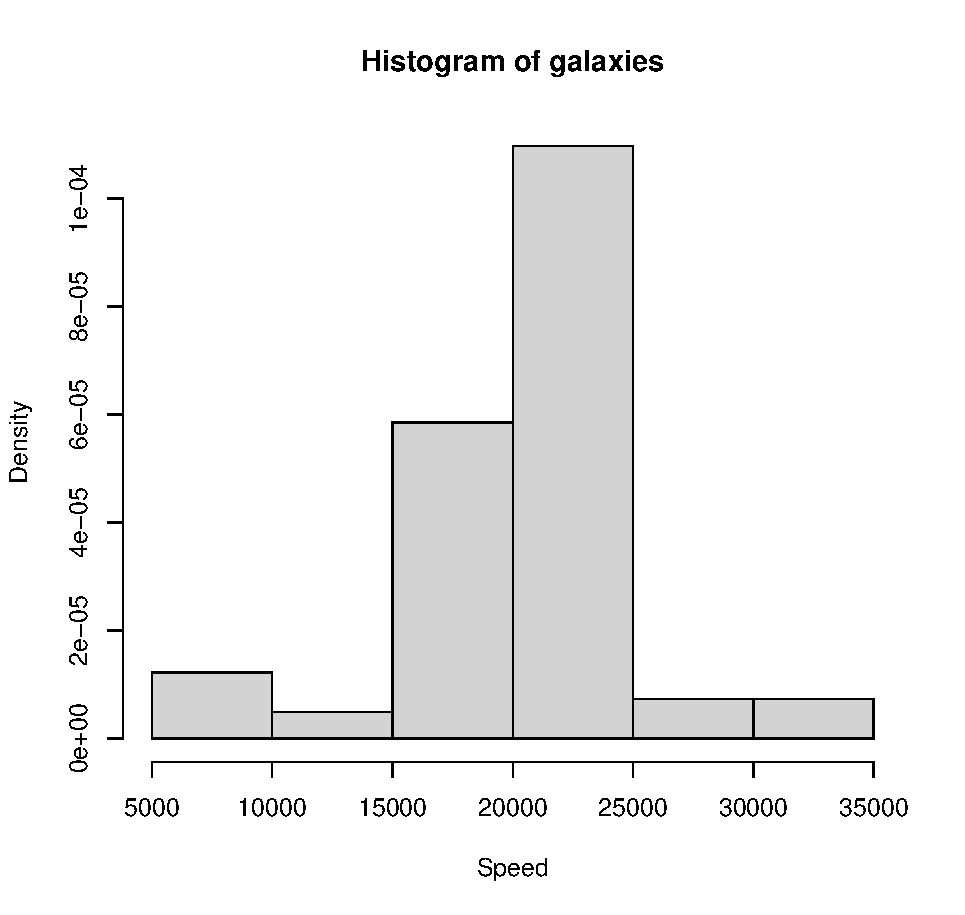
\includegraphics[scale=0.3]{figures/galaxies.pdf}
\end{center}
A now classical model is a Gaussian mixture:
\begin{equation*}
 \mathcal{M}_i : v_j \sim \sum_{l=1}^i p_{il} \cdot \operatorname{Normal}(v_j; \mu_{li},\sigma^2_{li}). 
\end{equation*}
\end{frame}
%%%%%%%%%%%%%%%%%%%%%%%%%%%%%%%%%%%
\begin{frame}{BMS: example III}
Consider the data:
 \begin{center}
 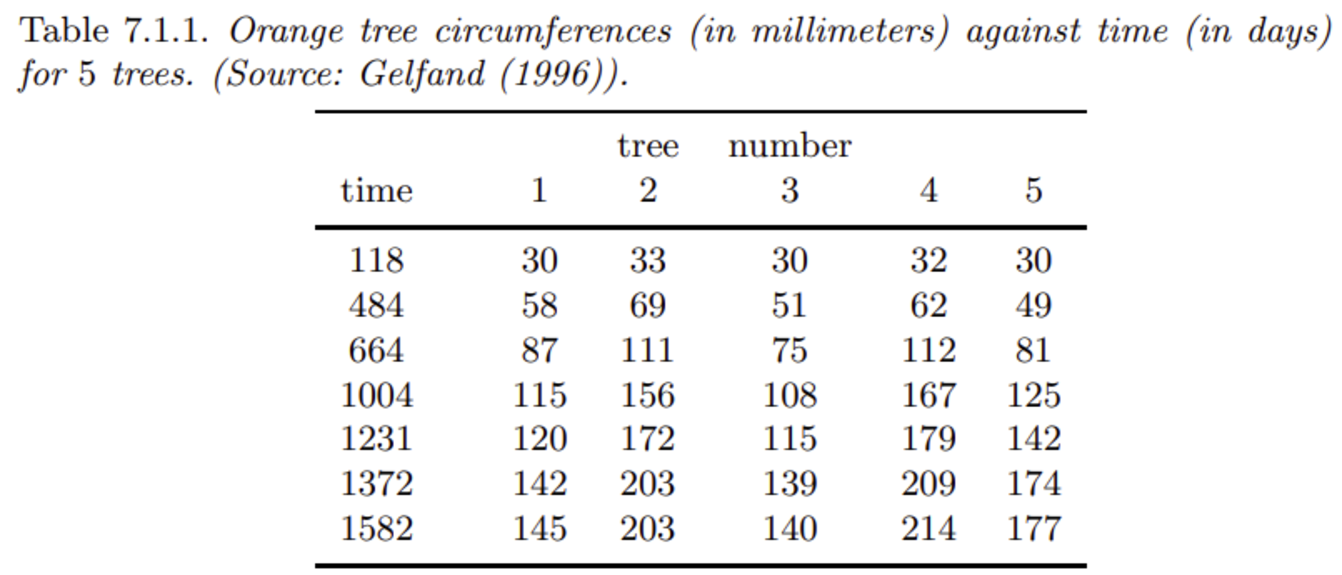
\includegraphics[scale=0.3]{figures/oranges.pdf}
\end{center}
Amongst the models we can consider, 
\begin{align*}
\mathcal{M}_1 :& y_{it} \sim \operatorname{Normal}(\beta_{10} + b_{1i}, \sigma_1^2), \\
\mathcal{M}_2 :& y_{it} \sim \operatorname{Normal}(\beta_{20} + \beta_{21}T_t + b_{2i}, \sigma_2^2) , \\
\mathcal{M}_3 :& y_{it} \sim \operatorname{Normal}\left(\frac{\beta_{30}}{1 + \beta_{31}\exp\left(\beta_{32} T_t\right)}, \sigma_3^2\right), \\
\mathcal{M}_4 :& y_{it} \sim \operatorname{Normal}\left(\frac{\beta_{40} + b_{4i}}{1 + \beta_{41}\exp\left(\beta_{42} T_t\right)}, \sigma_4^2\right).
\end{align*}
\end{frame}
%%%%%%%%%%%%%%%%%%%%%%%%%%%%%%%%%%%
\begin{frame}{Step 0: priors}
First, let us look at a convenient representation of model space:
\begin{equation*}
 \boldsymbol{\Theta} = \bigcup_{i \in I} \{i\} \times \boldsymbol{\Theta}_i.
\end{equation*}
Now, to each $\mathcal{M}_i$, we associate a prior $\pi_i(\theta_i)$  on each subspace and, by Bayes' theorem we get
\begin{align*}
 \pr(\mathcal{M}_i \mid x) & = \pr( \mu = i \mid x), \\ 
 &= \frac{w_i \int_{\boldsymbol{\Theta}_i} f_i(x\mid t_i)\pi_i(t_i)\,dt_i}{\sum_{j} w_j \int_{\boldsymbol{\Theta}_j} f_j(x\mid t_j)\pi_j(t_j)\,dt_j },
\end{align*}
where the $w_i$ are the \textbf{prior probabilities} for each model.
\end{frame}
%%%%%%%%%%%%%%%%%%%%%%%%%%%%%%%%%%%
\begin{frame}{An intuitive predictive}
A nice consequence of the formulation we just saw is that the predictive distribution looks quite intuitive:
\begin{align}
\nonumber
 p(\tilde{x} \mid \boldsymbol{x}) &= \sum_{j} w_j \int_{\boldsymbol{\Theta}_j} f_j(\tilde{x} \mid t_j) f_j(\boldsymbol{x}\mid t_j)\pi_j(t_j)\,dt_j,\\
 \label{eq:predictive_1}
 &= \sum_{j} \pr(\mathcal{M}_j \mid \boldsymbol{x}) m_j(\tilde{x}).
\end{align}
\end{frame}
%%%%%%%%%%%%%%%%%%%%%%%%%%%%%%%%%%%
\begin{frame}{Hello, my old friend}
Here, Bayes factors also play a central role:
\begin{align*}
 \operatorname{BF}_{12} &= \frac{\pr(\mathcal{M}_1 \mid x)}{\pr(\mathcal{M}_2 \mid x)}\bigg/\frac{\pr(\mathcal{M}_1)}{\pr(\mathcal{M}_2)},\\
  &= \frac{w_1^\prime \cdot w_2}{w_2^\prime \cdot w_1},
\end{align*}
with $w_i^\prime := \pr(\mathcal{M}_1 \mid x)$.
\end{frame}
%%%%%%%%%%%%%%%%%%%%%%%%%%%%%%%%%%%
\begin{frame}{Model averaging}
What if we simply \textbf{refuse} to select one model?
We can write
\begin{align}
 \nonumber
 p(\tilde{x} \mid \boldsymbol{x})  &= \int_{\boldsymbol{\Theta}} f(\tilde{x} \mid t) f(\boldsymbol{x}\mid t)\pi(t)\,dt,\\
 \nonumber
 &= \sum_{j} \int_{\boldsymbol{\Theta}_j} f_j(\tilde{x} \mid t_j) g(j, t_j \mid \boldsymbol{x})\,dt_j,\\
 \nonumber
 &= \sum_j p (\mathcal{M}_j \mid \boldsymbol{x}) \int_{\boldsymbol{\Theta}_j} f_j(\tilde{x} \mid t_j) p(t_j \mid \boldsymbol{x})\,dt_j,\\
 \label{eq:predictive_2}
  &= \sum_j w_j^\prime \int_{\boldsymbol{\Theta}_j} f_j(\tilde{x} \mid t_j) p(t_j \mid \boldsymbol{x})\,dt_j.
\end{align}
which is another version of the expression in (\ref{eq:predictive_1}).
\end{frame}
%%%%%%%%%%%%%%%%%%%%%%%%%%%%%%%%%%%
\begin{frame}{Model checking}
Modern Bayesian inference not only allows for, but actively encourages model interrogation and checking.
\begin{itemize}
 \item The central idea of \textbf{Leave-one-out cross-validation (LOO)} is to estimate the \textit{expected log pointwise predictive density for a new dataset}, elpd:
 \begin{equation*}
  \operatorname{elpd} = \sum_{i=1}^n \int m(\tilde{x}_i)\log p(\tilde{x}_i \mid \boldsymbol{x})\,d\tilde{x}_i.
 \end{equation*}
 See \cite{Vehtari2017}.
 \item With \textbf{Posterior predictive checks (PPCs)} we wish to compare  functions of the observed data, $f(\boldsymbol{x})$ with functions of the predictive distribution, $f(\boldsymbol{\tilde{x}})$.
  \begin{center}
 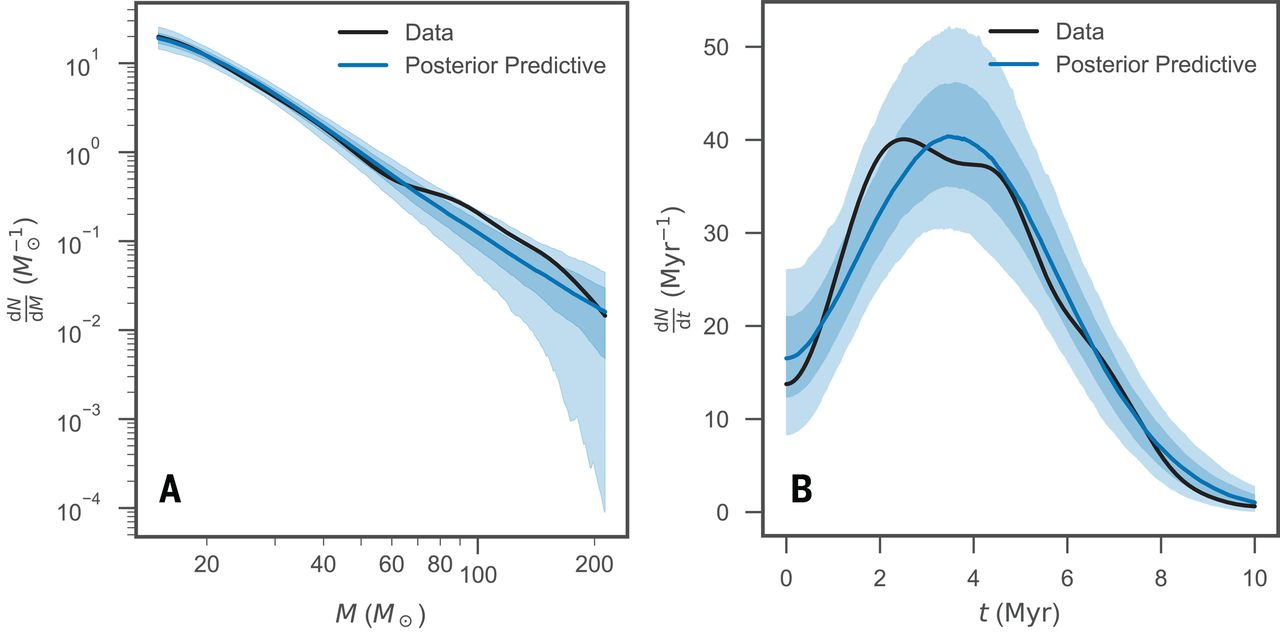
\includegraphics[scale=0.5]{figures/PPC.jpg}
\end{center}
 See \cite{Berkhof2000} and~\cite{Gabry2019}.
\end{itemize}
\end{frame}
%%%%%%%%%%%%%%%%%%%%%%%%%%%%%%%%%%%
\begin{frame}{Recommended reading}
\begin{itemize}
  \item[\faBook] \cite{Robert2007}, Ch. 7.
%  \item 
 \item[\faForward] Next lecture: \cite{Schervish1995} Ch. 7.4.
 \end{itemize} 
\end{frame}
